\documentclass[polish,polish,a4paper]{article}
\usepackage[T1]{fontenc}
\usepackage[utf8]{inputenc}
\usepackage{pslatex}
\usepackage{setspace}
\usepackage{caption}
\usepackage{amssymb}
\usepackage{amsmath}
\usepackage{anysize}
\usepackage{graphicx}
\usepackage{hyperref}
\usepackage{float}
\usepackage[polish]{babel}
\hypersetup{
	colorlinks=true,
	linkcolor=blue,
	filecolor=blue,      
	urlcolor=blue,
}

\marginsize{2.5cm}{2.5cm}{2cm}{2cm}


\begin{document}
	
\begin{spacing}{1.5}
		\begin{titlepage}
			\begin{flushright}
				{ Wtorki 16:50\\
					Grupa I3\\
					Kierunek Informatyka\\
					Wydział Informatyki\\
					Politechnika Poznańska}
			\end{flushright}
		\vspace*{\fill}
		\begin{center}
			{\Large Algorytmy i struktury danych \\[0.1cm]
				Sprawozdanie z zadania w zespołach nr. 1\\[0.1cm]
				prowadząca: dr hab. inż. Małgorzata Sterna, prof PP}\\[0.7cm]
			{\huge Algorytmy sortujące\\ [0.7cm]}
			{\large autorzy:\\[0.1cm]}
			{\large Piotr Więtczak nr indeksu 132339,\\[0.1cm] Tomasz Chudziak nr indeksu 136691}\\[0.5cm]
			\today
		\end{center}
		\vspace*{\fill}
	\end{titlepage}
	
	\section{Implementacja algorytmów sortujących}
	Do implementacji metod sortowania posłużyliśmy się językiem $ C++ $, każda metoda została napisana  w odrębnej  funkcji, która za parametry przyjmuje kolejno: wskaźnik na tablicę, rozmiar sortowanej tablicy oraz jako ostatni wartość opcjonalną “reverse” typu bool, która odpowiada za to czy tablica będzie posortowana rosnąco czy malejąco. Do mierzenia czasu poszczególnych metod użyliśmy klasy $ std::chrono::high::resolution\_clock  $ z biblioteki $ chrono $. Program użyty do obliczanie czasów sortowań, wraz z plikami nagłówkowymi zawierającymi metody sortujące, jest dostępny w formie repozytorium git pod adresem \hyperref{goo.gl/snMdzD}{}{}{goo.gl/snMdzD}.
	\section{Badana zależność czasu obliczeń $ t[s]$ od liczby sortowanych elementów~$ n $. }
	
	\subsection{Podział metod sortowania}
	W celu zachowania przejrzystości  otrzymanych danych podzieliliśmy metody na dwie grupy, "wolne" (Insertion Sort, Selection Sort, Bubble Sort) i $ " $szybkie$ " $ (Counting Sort, Quick Sort, Merge Sort, Heap Sort). Różnice w zależności czasu obliczeń $ t[s]$ od liczby sortowanych elementów~$ n $ dla algorytmów $ " $wolnych$ " $ i $ " $szybkich$ " $ przedstawiają poniższe wykresy.\\
	
	
\begin{minipage}[H]{\textwidth}
	\centering
	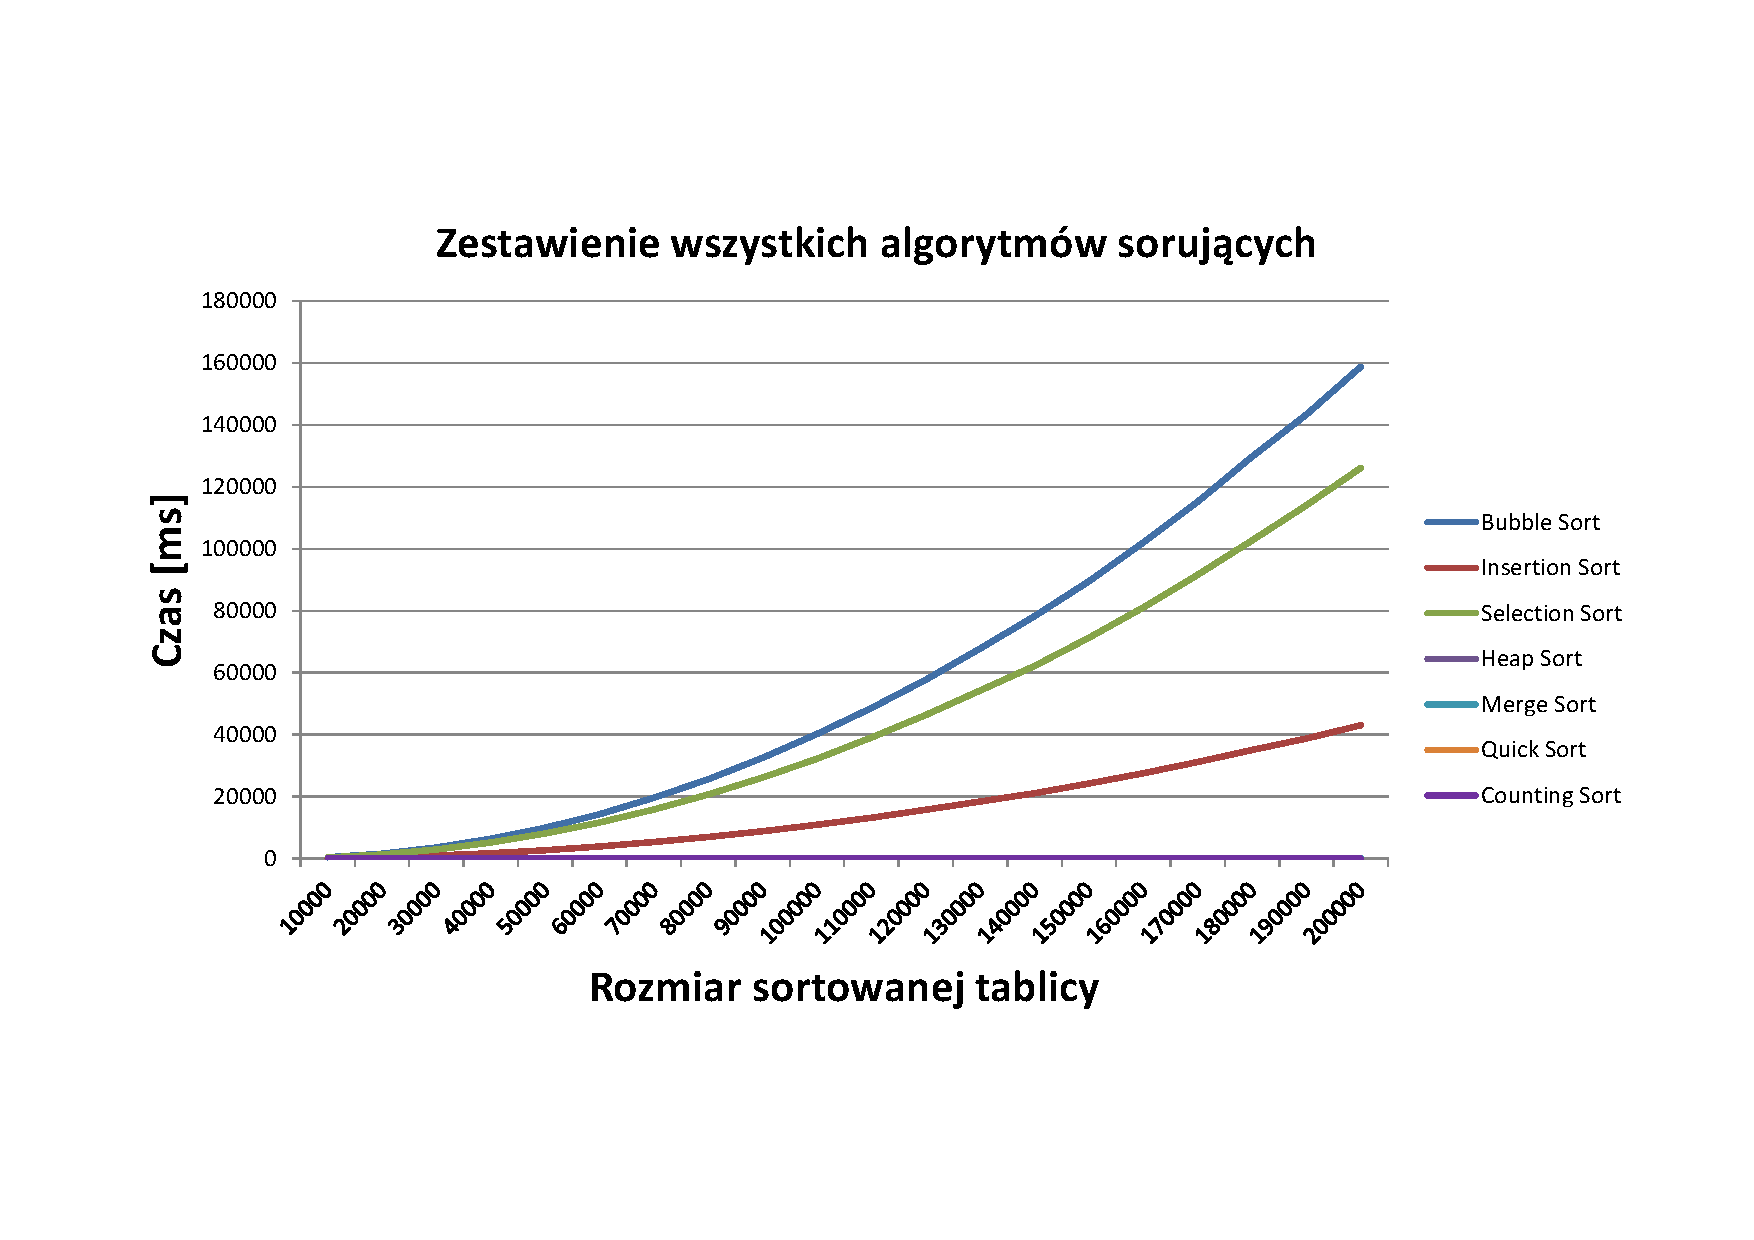
\includegraphics[scale=0.6]{zad2wsznor.pdf}
	\label{fig:2wszn}
\end{minipage}

\begin{minipage}[H]{\textwidth}
	\centering
	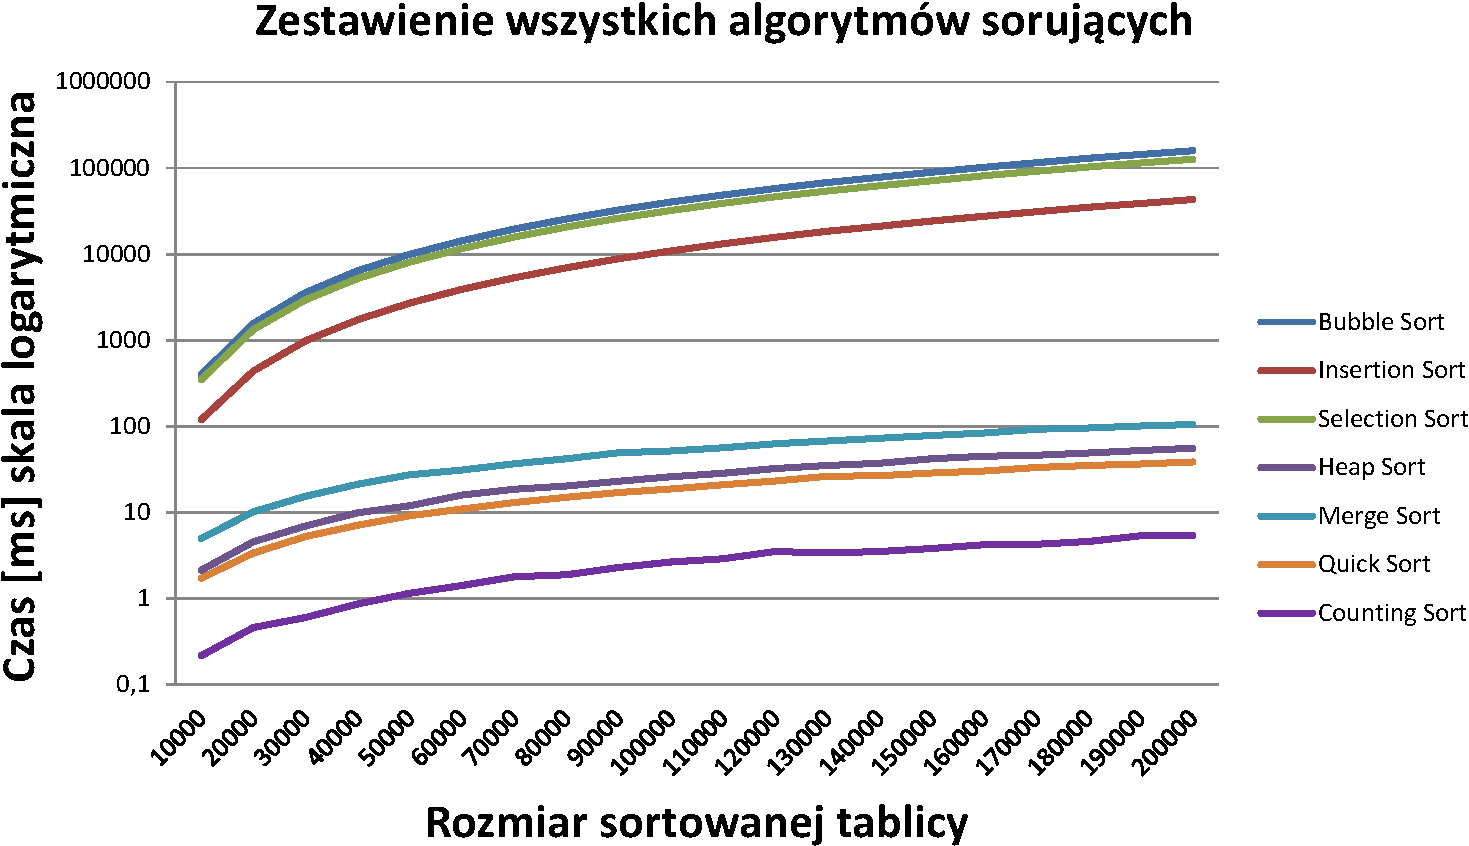
\includegraphics[scale=0.6]{zad2wszlog.pdf}
	\label{fig:2wszl}
\end{minipage}
	
	\subsection*{Wnioski do podziału metod sortowania}
	
	Jak widać na \hyperref[fig:2wszn]{wykresie} przedstawiajacym zależność czasu obliczeń od liczby sortowanych elementów, linie przedstawiające metody $ " $szybkie$ " $ zlewają się ze sobą i leżą przy samej osi OX, \hyperref[fig:2wszn]{wykres} pokazuje także jak znacząca jest różnica szybkości wykonywania sortowań między grupami. Dopiero przedstawienie danych na \hyperref[fig:2wszl]{wykresie} ze skalą logarytmiczną pozwala rozróżnić metody $"$szybkie$"$.
	
	\subsection{Metody $ "$wolne$" $}
	\subsubsection{Opis algorytmów $"$wolnych$"$}
	\subsubsection*{Insertion Sort (sortowanie przez wstawianie)}
	Polega na wstawieniu kolejnego elementu z nieposortowanej części tablicy odpowiednie miejsce w posortowanej części tablicy.\\
	
	Zalety:
	\begin{itemize}
		\item wydajny dla zbiorów wstępnie posortowanych
		\item działa w miejscu
		\item stabilny 
	\end{itemize}
	Wady:
	\begin{itemize}
		\item wolniejszy od metod $ " $szybkich$ " $
		\item mało wydajne dla dużej ilości elementów do posortowania
	\end{itemize}
	Inne cechy:
	\begin{itemize}
		\item zachowanie naturalne
	\end{itemize}
	
				\subsubsection*{Tabela przedstawiająca złożoność obliczeniową dla przypadków optymistycznego, średniego i pesymistycznego} 
	
	\begin{figure}[H]
		\begin{equation*}
		\begin{array}{l|c|c|c|}

		&$złożoność obliczeniowa$&$złożoność obliczeniowa$&$złożoność obliczeniowa$\\
		&$dla przypadku$&$dla przypadku$&$dla przypadku$\\
		&$optymistycznego$&$średniego$&$pesymistycznego$\\
		\hline
		$Insert Sort$&O(n^2)&O(n^2)&O(n^2)\\
		\hline
		\end{array}
		\end{equation*}
		\captionof{table}{Tablica złożoności obliczeniowej dla metody Insert Sort}
	\end{figure}
		
		\subsubsection*{Selection Sort (sortowanie przez wybieranie)}
		Polega na wyszukaniu w nieposortowanej części tablicy elementu który powinien się znaleźć w pożądanym miejscu i zamianie miejscami z tym który obecnie się tam znajduje.\\
		
	Zalety:
	\begin{itemize}
		\item działa w miejscu
		\item stabilny 
	\end{itemize}
	Wady:
	\begin{itemize}
		\item wolniejszy od metod $ " $szybkich$ " $
		\item mało wydajne dla dużej ilości elementów do posortowania
	\end{itemize}
	Inne cechy:
	\begin{itemize}
		\item zachowanie naturalne
	\end{itemize}
	
				\subsubsection*{Tabela przedstawiająca złożoność obliczeniową dla przypadków optymistycznego, średniego i pesymistycznego} 
	\begin{figure}[H]

		\begin{equation*}
		\begin{array}{l|c|c|c|}

		&$złożoność obliczeniowa$&$złożoność obliczeniowa$&$złożoność obliczeniowa$\\
		&$dla przypadku$&$dla przypadku$&$dla przypadku$\\
		&$optymistycznego$&$średniego$&$pesymistycznego$\\
		\hline
		$Selection Sort$&O(n^2)&O(n^2)&O(n^2)\\
		\hline
		\end{array}
		\end{equation*}
		\captionof{table}{Tablica złożoności obliczeniowej dla metody Selection Sort}
	\end{figure}
	
	
			\subsubsection*{Bubble Sort (sortowanie bąbelkowe)}
			Polega na porównaniu dwóch kolejnych elementów i zamianie ich kolejności, jeśli nie pasuje ona do porządku sortowania tablicy. Sortowanie kończy się kiedy podczas przejścia nie dokonano żadnej zmiany.\\
			
	Zalety:
	\begin{itemize}
		\item działa w miejscu
		\item stabilny 
	\end{itemize}
	Wady:
	\begin{itemize}
		\item wolniejszy od metod $ " $szybkich$ " $
		\item mało wydajne dla dużej ilości elementów do posortowania
	\end{itemize}
	Inne cechy:
	\begin{itemize}
		\item zachowanie naturalne
	\end{itemize}
	
	
	\subsubsection*{Tabela przedstawiająca złożoność obliczeniową dla przypadków optymistycznego, średniego i pesymistycznego} 
	
	\begin{figure}[H]
			\begin{equation*}
		\begin{array}{l|c|c|c|}

		&$złożoność obliczeniowa$&$złożoność obliczeniowa$&$złożoność obliczeniowa$\\
		&$dla przypadku$&$dla przypadku$&$dla przypadku$\\
		&$optymistycznego$&$średniego$&$pesymistycznego$\\
		\hline
		$Bubble Sort$&O(n^2)&O(n^2)&O(n^2)\\
		\hline
		\end{array}
		\end{equation*}
		\captionof{table}{Tablica złożoności obliczeniowej dla metody Bubble Sort}
	\end{figure}

	\subsubsection*{Tabela ilustrująca zależności czasu sortowania od ilości elementów dla metod $"$wolnych$"$, zakres liczb $ [1,n] $.}
	
	\begin{figure}[H]
			\begin{equation*}
		\begin{array}{l|c|c|c|}

		$Liczba elem.$&$Insertion Sort$&$Selection Sort$&$Bubble Sort$\\\hline
		10000&	116,367&	343,188&	399,54\\\hline
		20000&	443,897&	1353,49&	1553,66\\\hline
		30000&	1031,43&	3012&	3594,1\\\hline
		40000&	1729,67&	5245,04&	6400,49\\\hline
		50000&	2736,71&	8192,25&	9928,66\\\hline
		60000&	3893,3&	11588,5&	14420,7\\\hline
		70000&	5305&	15701,2&	19430,2\\\hline
		80000&	6920,76&	20416,9&	25364,5\\\hline
		90000&	8782,01&	25847,5&	32131,7\\\hline
		100000&	10820,4&	31732,1&	39683,9\\\hline
		110000&	13004,1&	38229,9&	47605\\\hline
		120000&	15467&	45476,8&	56842,2\\\hline
		130000&	18181,8&	53262,1&	66675,1\\\hline
		140000&	21019,3&	61749&	77105,2\\\hline
		150000&	24263,4&	70873,2&	88830,4\\
		\hline
		\end{array}
		\end{equation*}
		\captionof{table}{Wyniki badań zależności czasu od iloci elementów dla metod $"$wolnych$"$}
	\end{figure}
	
	\subsubsection*{Wykres ilustrujący zależności czasu sortowania od ilości elementów dla metod $"$wolnych$"$, zakres liczb $ [1,n] $.}
	
	\begin{minipage}[H]{\textwidth}
		\begin{center}
					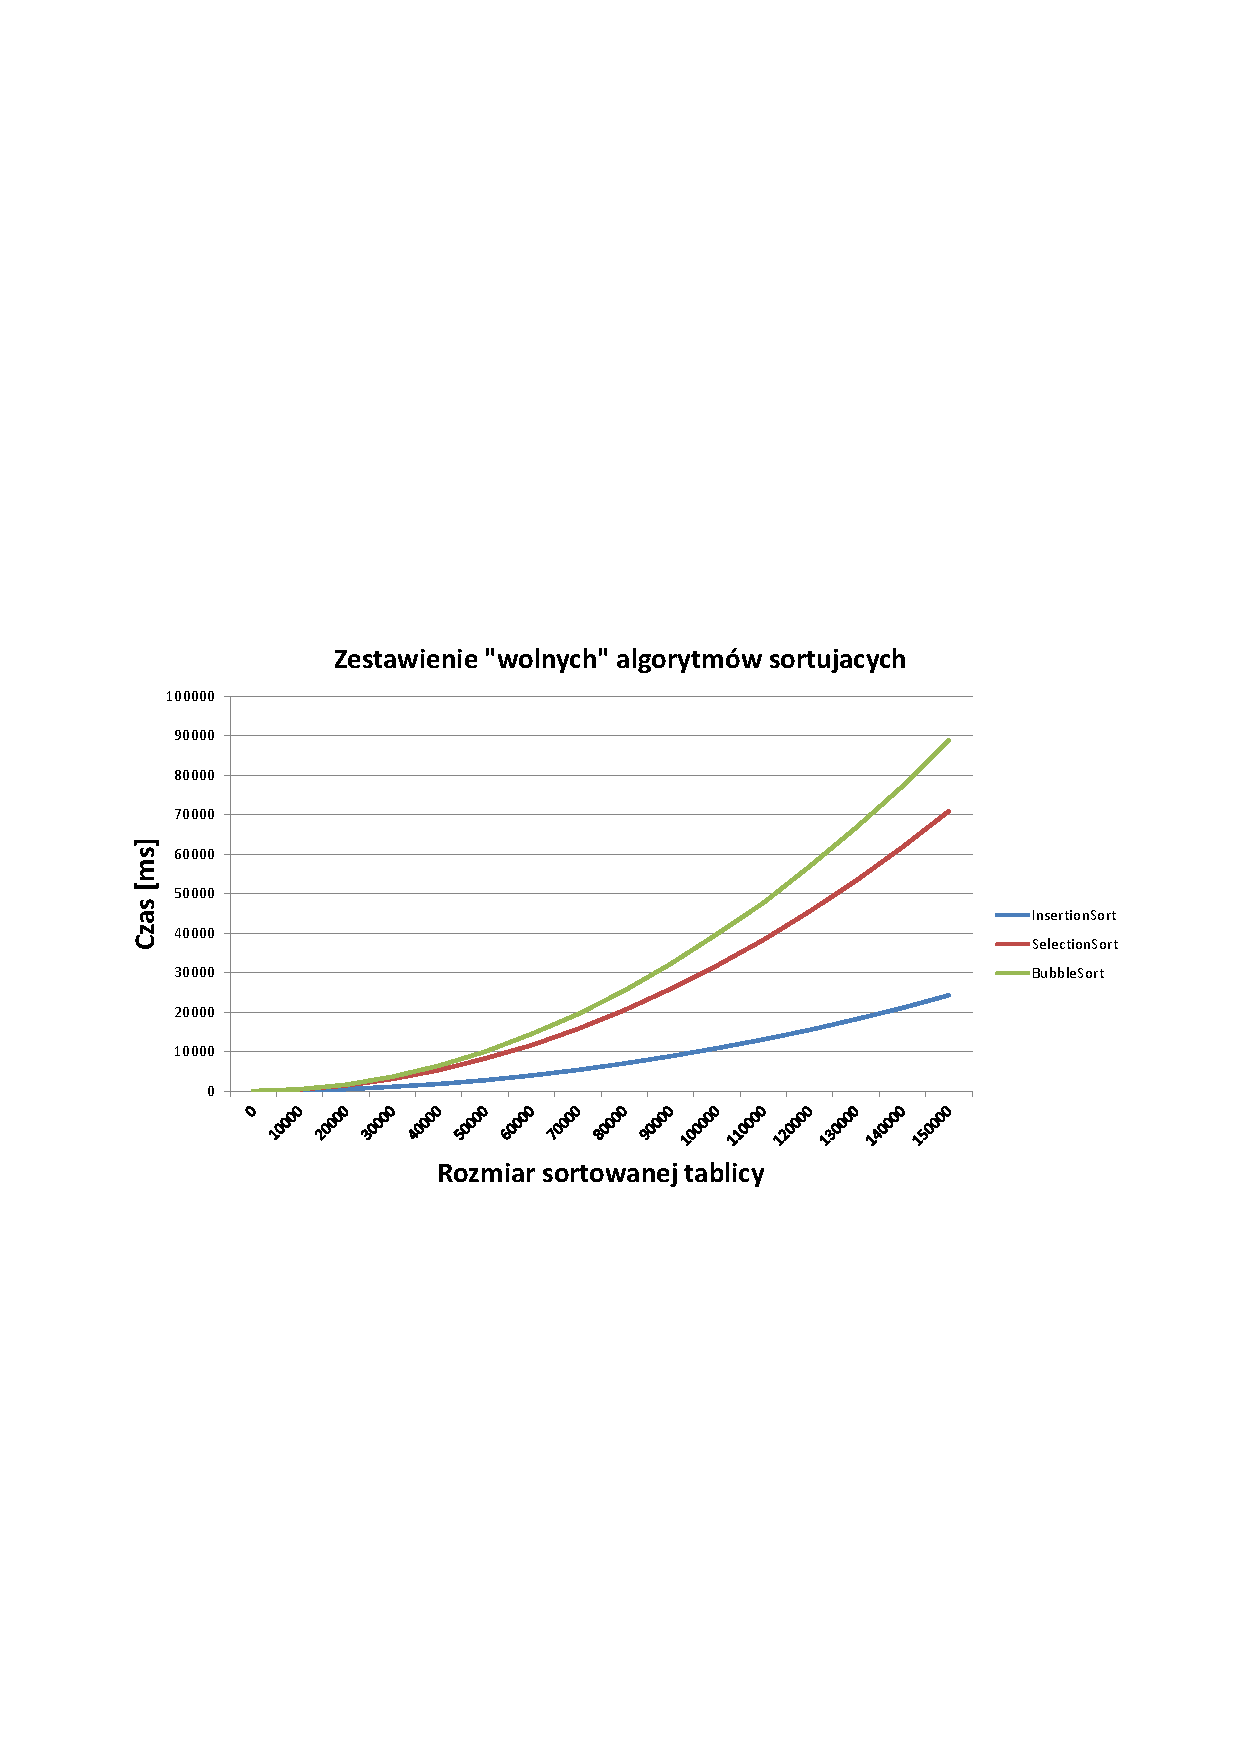
\includegraphics[scale=0.85]{zad2wolne.pdf}
					\label{fig:zad2wolne}
		\end{center}
	\end{minipage}

\subsubsection{Wnioski do metod $"$wolnych$"$}

Metody $"$wolne$"$, są zwykle o wiele mniej efektywne od metod $"$szybkich$"$, a wraz z wzrostem ilości elementów do posortowania dysproporcja się pogłębia.
	
	\subsection{Metody $"$szybkie$"$}

	\subsubsection{Opis algorytmów $"$szybkich$"$}

		\subsubsection*{Quick Sort (sortowanie szybkie)}
		Działanie algorytmu zaczyna się od wybrania elementu podziału, w badanej przez nas implementacji był to element środkowy, następnie tablica zostaje podzielona na dwie części, do początkowej przenoszone są wszystkie elementy mniejsze od elementu podziału, nie mniejsze trafiają natomiast do końcowej części. Następnie algorytm sortuje osobno w ten sam sposób części początkową i końcową. Warunkiem końcowym rekursji będzie uzyskanie w wyniku podziału tylko jednego elementu, jednoelementowa tablica nie wymaga sortowania.\\
		
	Zalety:
	\begin{itemize}
		\item działa w miejscu
	\end{itemize}
	Wady:
	\begin{itemize}
		\item niestabilny
		\item wrażliwy na dane wejściowe 
	\end{itemize}
	Inne cechy:
	\begin{itemize}
		\item zachowanie nienaturalne
		\item korzysta z metody $"$dziel i rządź$"$
		\item algorytm rekurencyjny
	\end{itemize}
	
	\subsubsection*{Tabela przedstawiająca złożoność obliczeniową dla przypadków optymistycznego, średniego i pesymistycznego} 
	\begin{figure}[H]
		
		\begin{equation*}
		\begin{array}{l|c|c|c|}

		&$złożoność obliczeniowa$&$złożoność obliczeniowa$&$złożoność obliczeniowa$\\
		&$dla przypadku$&$dla przypadku$&$dla przypadku$\\
		&$optymistycznego$&$średniego$&$pesymistycznego$\\
		\hline
		$Quick Sort$&O(n\log_{2}(n))&O(n\log_{2}(n))&O(n^2)\\
		\hline
		\end{array}
		\end{equation*}
		\captionof{table}{Tablica złożoności obliczeniowej dla metody Quick Sort}
	\end{figure}
	
			\subsubsection*{Merge Sort (sortowanie przez scalanie)}
			Działanie metody polega na podzieleniu sortowanej tablicy na dwie równe części (jeżeli to możliwe), następnie algorytm zostaje użyty ponownie osobno dla obu części podziału, zagłębianie rekursji trwa do momentu aż do podzielenia pozostanie tylko jeden element. Na koniec powracając z rekurencji metoda łączy posortowane podciągi w jeden ciąg posortowany.\\
			
	Zalety:
	\begin{itemize}
		\item algorytm asymptotycznie optymalny
		\item stabilny
		\item niewrażliwy na dane wejściowe
	\end{itemize}
	Wady:
	\begin{itemize}
		\item nie działa w miejscu
	\end{itemize}
	Inne cechy:
	\begin{itemize}
		\item zachowanie nienaturalne
		\item korzysta z metody $"$dziel i rządź$"$
		\item algorytm rekurencyjny
	\end{itemize}
	
	\subsubsection*{Tabela przedstawiająca złożoność obliczeniową dla przypadków optymistycznego, średniego i pesymistycznego} 
	\begin{figure}[H]
		
		\begin{equation*}
		\begin{array}{l|c|c|c|}

		&$złożoność obliczeniowa$&$złożoność obliczeniowa$&$złożoność obliczeniowa$\\
		&$dla przypadku$&$dla przypadku$&$dla przypadku$\\
		&$optymistycznego$&$średniego$&$pesymistycznego$\\
		\hline
		$Merge Sort$&O(n\log_{2}(n))&O(n\log_{2}(n))&O(n^2)\\
		\hline
		\end{array}
		\end{equation*}
		\captionof{table}{Tablica złożoności obliczeniowej dla metody Merge Sort}
	\end{figure}
	
			\subsubsection*{Heap Sort (sortowanie przez kopcowanie)}
			Działanie metody wykorzystuje strukturę binarnego kopca zupełnego. Po utworzeniu z tablicy do posortowania kopca następuje sortowanie, polega ono na zamianę miejscami korzenia kopca z ostatnim elementem i odbudowie kopca bez udziału elementów wcześniej przeniesionych na koniec tablicy. Operację powtarza się do momentu wyczerpania elementów kopca. W ten sposób w części która nie bierze ponownego udziału w kopcowaniu powstaje posortowana tablica.\\
						
Zalety:
\begin{itemize}
	\item działa w miejscu
	\item  mało wrażliwy na dane wejściowe
\end{itemize}
Wady:
\begin{itemize}
	\item niestabilny

\end{itemize}
Inne cechy:
\begin{itemize}
	\item zachowanie nienaturalne
	\item korzysta ze stogów
\end{itemize}

\subsubsection*{Tabela przedstawiająca złożoność obliczeniową dla przypadków optymistycznego, średniego i pesymistycznego} 
\begin{figure}[H]
	
	\begin{equation*}
	\begin{array}{l|c|c|c|}

	&$złożoność obliczeniowa$&$złożoność obliczeniowa$&$złożoność obliczeniowa$\\
	&$dla przypadku$&$dla przypadku$&$dla przypadku$\\
	&$optymistycznego$&$średniego$&$pesymistycznego$\\
	\hline
	$Heap Sort$&O(n)&kek&O(n\log_{2}(n))\\
	\hline
	\end{array}
	\end{equation*}
	\captionof{table}{Tablica złożoności obliczeniowej dla metody Heap Sort}
\end{figure}

			\subsubsection*{Counting Sort (sortowanie przez zliczanie)}
			
			Polega na sprawdzeniu ile razy w tablicy wystąpił element z sortowanego zakresu, następnie algorytm sprawdza ile wystąpień elementów mniejszych od danego w występuje w sortowanej tablicy, na koniec wypisuje posortowany ciąg do tablicy wynikowej. Metoda zakłada, że elementy tablicy należą do liczb całkowitych nieujemnych.\\
			
Zalety:
\begin{itemize}
	\item bardzo szybki algorytm sortowania dla danych z małego zakresu
	\item stabilny
\end{itemize}
Wady:
\begin{itemize}
	\item nie działa w miejscu
	\item ograniczony ze względu na zakres sortowanych liczb
	\item mało wydajny dla danych z dużego przedziału
\end{itemize}


\subsubsection*{Tabela przedstawiająca złożoność obliczeniową dla przypadków optymistycznego, średniego i pesymistycznego} 
\begin{figure}[H]
	
	\begin{equation*}
	\begin{array}{l|c|c|c|}

	&$złożoność obliczeniowa$&$złożoność obliczeniowa$&$złożoność obliczeniowa$\\
	&$dla przypadku$&$dla przypadku$&$dla przypadku$\\
	&$optymistycznego$&$średniego$&$pesymistycznego$\\
	\hline
	$Counting Sort$&O(n)&O(n)&O(n)\\
	\hline
	\end{array}
	\end{equation*}
	\captionof{table}{Tablica złożoności obliczeniowej dla metody Counting Sort}
\end{figure}

	\subsubsection*{Tabela ilustrująca zależności czasu sortowania od ilości elementów dla metod $"$szybkich$"$, zakres liczb $ [1,n] $.}

\begin{figure}[H]
	\begin{equation*}
	\begin{array}{l|c|c|c|c|}
	
	$Liczba elem.$&$Counting Sort$&$Heap Sort$&$Merge Sort$&$Quick Sort$\\\hline
	1000000&	85,9862& 441,528& 599,972&	223,697\\\hline
	2000000& 204,386&	790,249&	1168,86&	459,433\\\hline
	3000000&	344,066&	1281,85&	1781,07&	698,22\\\hline
	4000000& 480,98&	1793,7&	2373,11&	938,052\\\hline
	5000000& 617,621&	2358,77&	3014,62&	1185,58\\\hline
	6000000& 756,102&	2902,17&	3626,7&	1433,96\\\hline
	7000000& 901,962&	3486,93&	4246,06&	1675,53\\\hline
	8000000& 1043,01&	4115,85&	4843,67&	1947,04\\\hline
	9000000& 1200,79&	4700,67&	5490,97&	2185,94\\\hline
	10000000& 	1347,63&	5347,84&	6139,22&	2446,77\\\hline
	11000000& 	1503,04&	5980,28&	6791,13&	2704,96\\\hline
	12000000& 	1649,68&	6614,99&	7416,89&	2969,83\\\hline
	13000000& 	1803,17&	7291,14&	8067,89&	3210,14\\\hline
	14000000& 	1961,38&	7964,01&	8694,71&	3489,29\\\hline
	15000000& 	2114,89&	8658,49&	9302,72&	3724,19\\\hline
	16000000& 	2269,11&	9285,66&	9908&	4032,19\\\hline
	17000000& 	2432,23&	9984,3&	10570,9&	4258,68\\\hline
	18000000& 	2597,7&	10655,1&	11213,5&	4489,62\\\hline
	19000000& 	2740,3&	11530,3&	11864,9&	4786,57\\\hline
	20000000& 	2896,79&	12065,7&	12529,9&	5046,56\\
	\hline

	\end{array}
	\end{equation*}
	\captionof{table}{Wyniki badań zależności czasu od iloci elementów dla metod $"$szybkich$"$}
\end{figure}

\subsubsection*{Wykres ilustrujący zależności czasu sortowania od ilości elementów dla metod $"$szybkich$"$, zakres liczb $ [1,n] $.}

	\begin{minipage}[H]{\textwidth}
	\begin{center}
		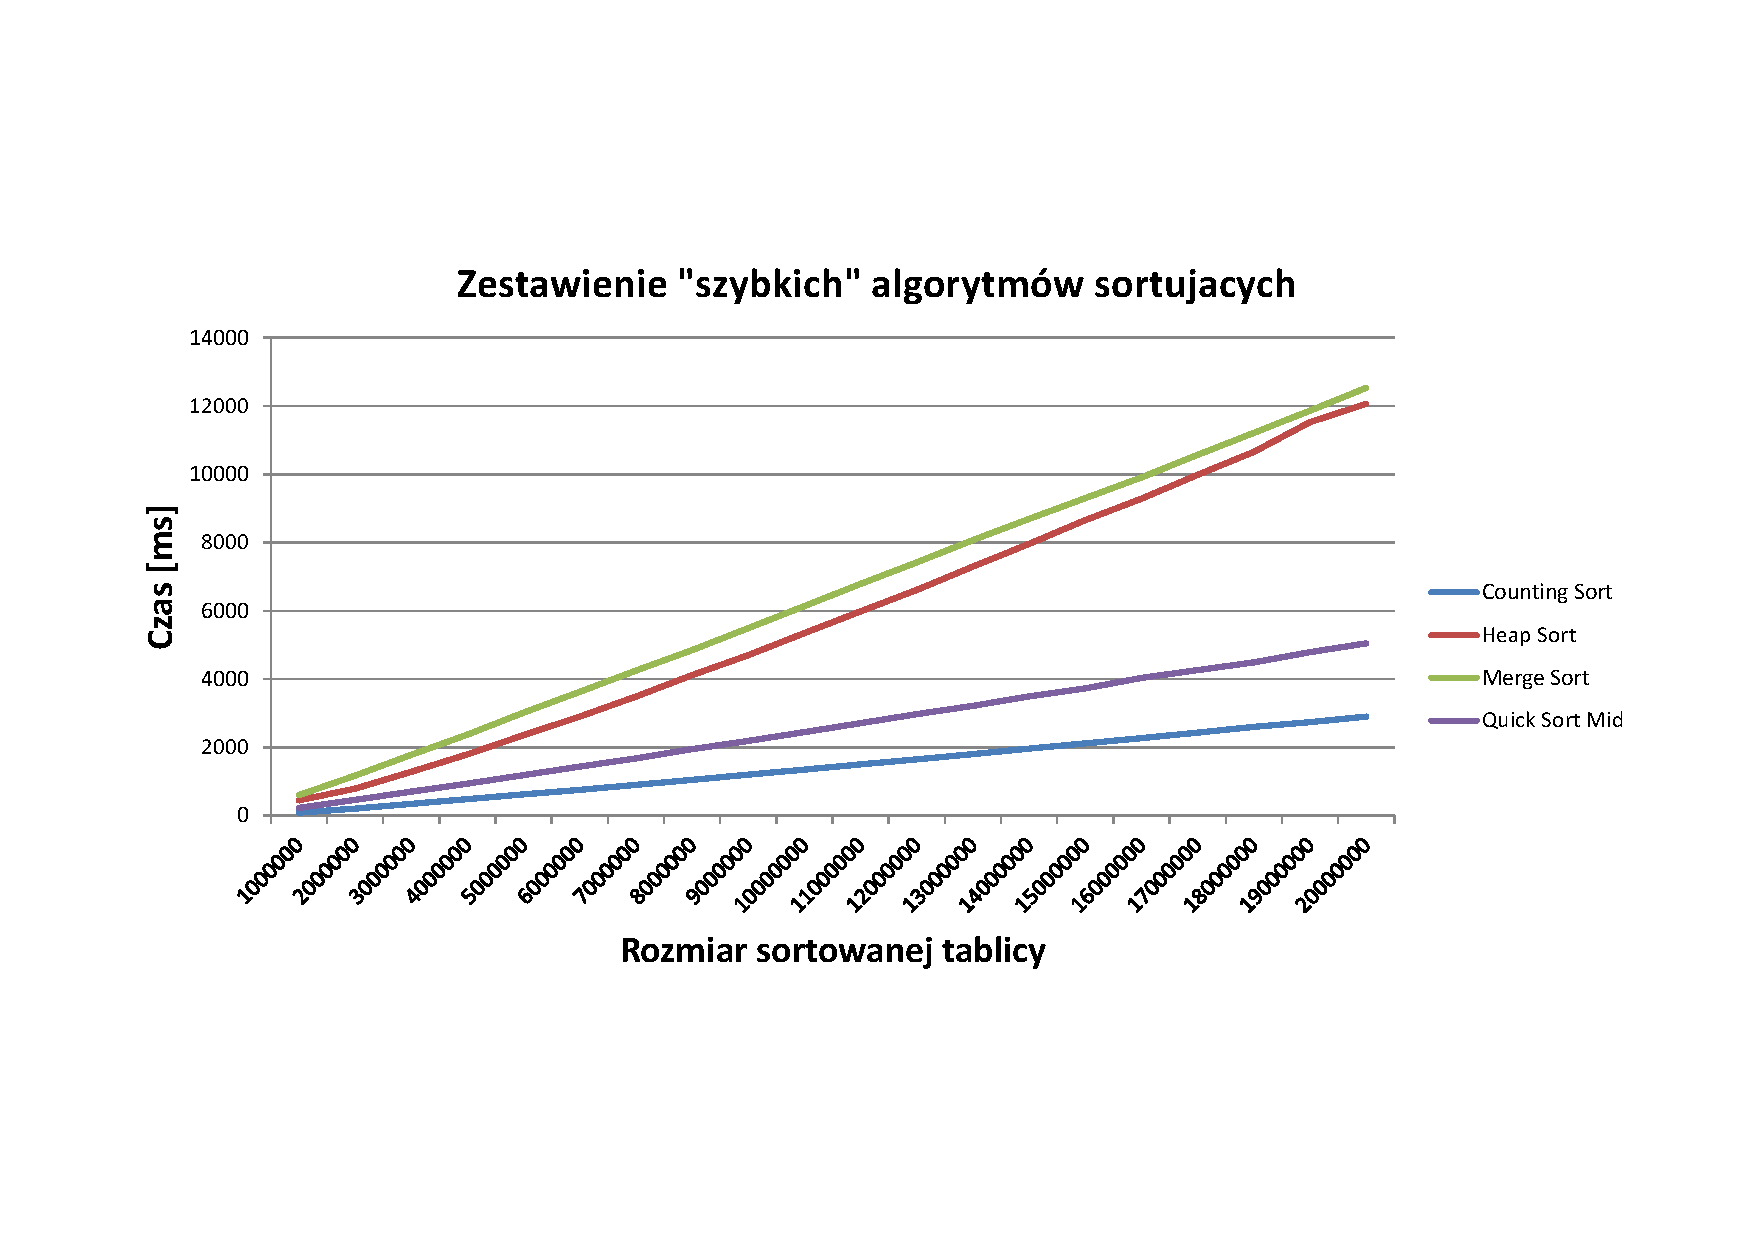
\includegraphics[scale=0.6]{zad2szybkie.pdf}
		\label{fig:zad2szybkie}
	\end{center}
\end{minipage}

\subsubsection{Wnioski do metod $"$szybkich$"$}

Metody $"$szybkie$"$ są zwykle bardziej efektywne od metod $"$wolnych$"$, nie ma to jednak zawsze miejsca o czym przekonamy się dalszej części sprawozdania.


\subsection{Wnioski do podziału metod sortowania}

Dzieląc metody sortowania można brać pod wiele rzeczy takich jak: czas wykonywania, dodatkowe zużycie pamięci, czy wrażliwość na dane wejściowe i wiele innych. Najczęściej wyróżnia się jednak podział ze względu na właśnie te trzy czyniki, na metody $ " $szybkie$ " $ (Counting Sort, Merge Sort, Quick Sort, Heap Sort) i $"$wolne$"$ (Insertion Sort, Selection Sort, Bubble Sort), ale także na pracujące w miejscu (Insertion Sort, Selection Sort, Bubble Sort, Heap Sort, Quick Sort) i wymagające dodatkowej pamięci (Merge Sort, Counting Sort), oraz wrażliwe na dane wejściowe (Quick Sort) , mało wrażliwe na dane wejściowe (Insertion Sort, Bubble Sort, Selection Sort, Counting Sort, Heap Sort) i niewrażliwe na dane wejściowe (Merge Sort). Więcej o czynikach wspomagających wybór metody sortowania powiemy we wnioskach do sekcji 3.


\section{Badanie zależności czasu $t$ od liczby sortowanych elementów $n$, przy rozkładach losowych i rosnących, dla metod Quick Sort z podziałem wg: skrajnego i środowego elementu, oraz dla metody Insert Sort}

W dalszej części sprawozdania algorytm Quick Sort z podziałem według środkowego elementu będziemy nazywać Quick Sort Mid, a z podziałem według skrajnego elementu Qick Sort Right.


	\subsubsection*{Tabela ilustrująca zależności czasu sortowania od ilości elementów dla metod Quick Sort Mid, Quick Sort Right, Insertion Sort, dla rozkładów losowego i rosnącego.}


\begin{figure}[H]
	\begin{equation*}
	\begin{array}{l|c|c|c|c|c|c|}
	
	&$Insert Sort$&$Quick Sort R$&$Quick Sort M$&$Insert Sort$&$Quick Sort R$&$Quick Sort M$\\
	$Liczba. elem.$&$roz. losowy$&$roz. losowy$&$roz. losowy$&$roz.rosnący$&$roz. rosnący$&$roz. rosnący$\\\hline
	10000&	113,203&	1,6697&	1,76432&	0,032714&	155,83&	0,838059\\\hline
	20000&	437,488&	3,39137&	3,60882&	0,065428&	509,5&	1,72166\\\hline
	30000&	984,901&	5,20155&	5,21053&	0,096218&	969,508&	2,61136\\\hline
	40000&	1735,75&	7,16728&	7,09833&	0,127649&	1590,15&	3,52479\\\hline
	50000&	2702,44&	9,20614&	9,80398&	0,156515&	2498,85&	4,63739\\\hline
	60000&	3912,19&	11,4185&	11,567&	0,195002&	3675,9&	5,46967\\\hline
	70000&	5331,38&	13,4157&	12,9942&	0,217132&	4884,01&	6,15699\\\hline
	80000&	6932,69&	15,1264&	15,5626&	0,265882&	6331,66&	7,15702\\\hline
	90000&	8767,07&	16,623&	16,5934&	0,31335&	7946&	8,44217\\\hline
	100000&	10802,7&	18,4383&	18,6365&	0,331311&	9934,8&	9,62822\\\hline
	110000&	13141,5&	20,523&	21,3091&	0,351517&	11940&	9,6619\\\hline
	120000&	15639,8&	22,4413&	22,4955&	0,386476&	13993,6&	10,8232\\\hline
	130000&	18263,4&	24,3281&	24,3358&	0,409889&	16322,7&	11,2511\\\hline
	140000&	21317,5&	26,8089&	26,5324&	0,425926&	18797&	11,8903\\\hline
	150000&	24363,9&	28,5161&	28,5139&	0,459281&	21520,3&	13,2566\\\hline
	160000&	27679&	31,3674&	31,224&	0,505466&	24480,6&	14,1598\\\hline
	170000&	31397,9&	32,184&	32,2783&	0,535934&	27719,3&	15,5934\\\hline
	180000&	35062,8&	35,0455&	34,6744&	0,54748&	31037,2&	16,4565\\\hline
	190000&	38904,7&	36,609&	36,2957&	0,586288&	34542,1&	19,0432\\\hline
	200000&	43261,1&	39,1665&	40,5784&	0,701429&	38319,8&	19,7654\\
	
	\hline
	\end{array}
	\end{equation*}
	\captionof{table}{Wyniki badań zależności czasu od ilości elementów dla metod Quick Sort M (z podziałem według środkowego elementu), Quick Sort R (z podziałem według skrajnego elementu), Insertion Sort, dla rozkładów losowego i rosnącego.}
\end{figure}

\subsection{Rozkład losowy}

\subsubsection*{Wykresy ilustrujące zależności czasu sortowania od ilości elementów dla metod Quick Sort Mid, Quick Sort Right, Insertion Sort, dla rozkładu losowego.}




\begin{minipage}[H]{\textwidth}
	\begin{center}
		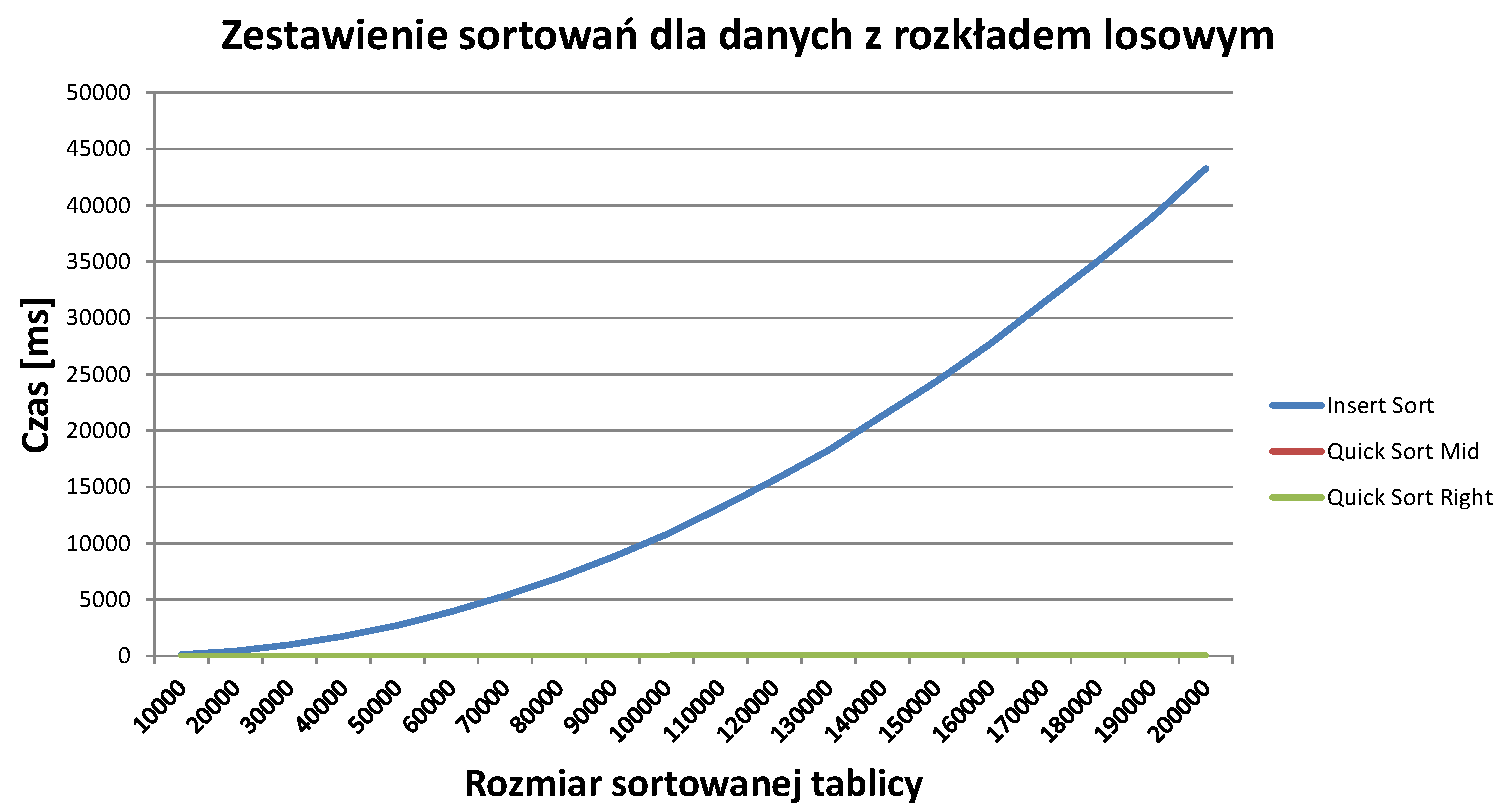
\includegraphics[scale=0.6]{zad3losowynorm.pdf}
		\label{fig:zad3losn}
	\end{center}
\end{minipage}\\[1cm]



\begin{minipage}[H]{\textwidth}
	\begin{center}
		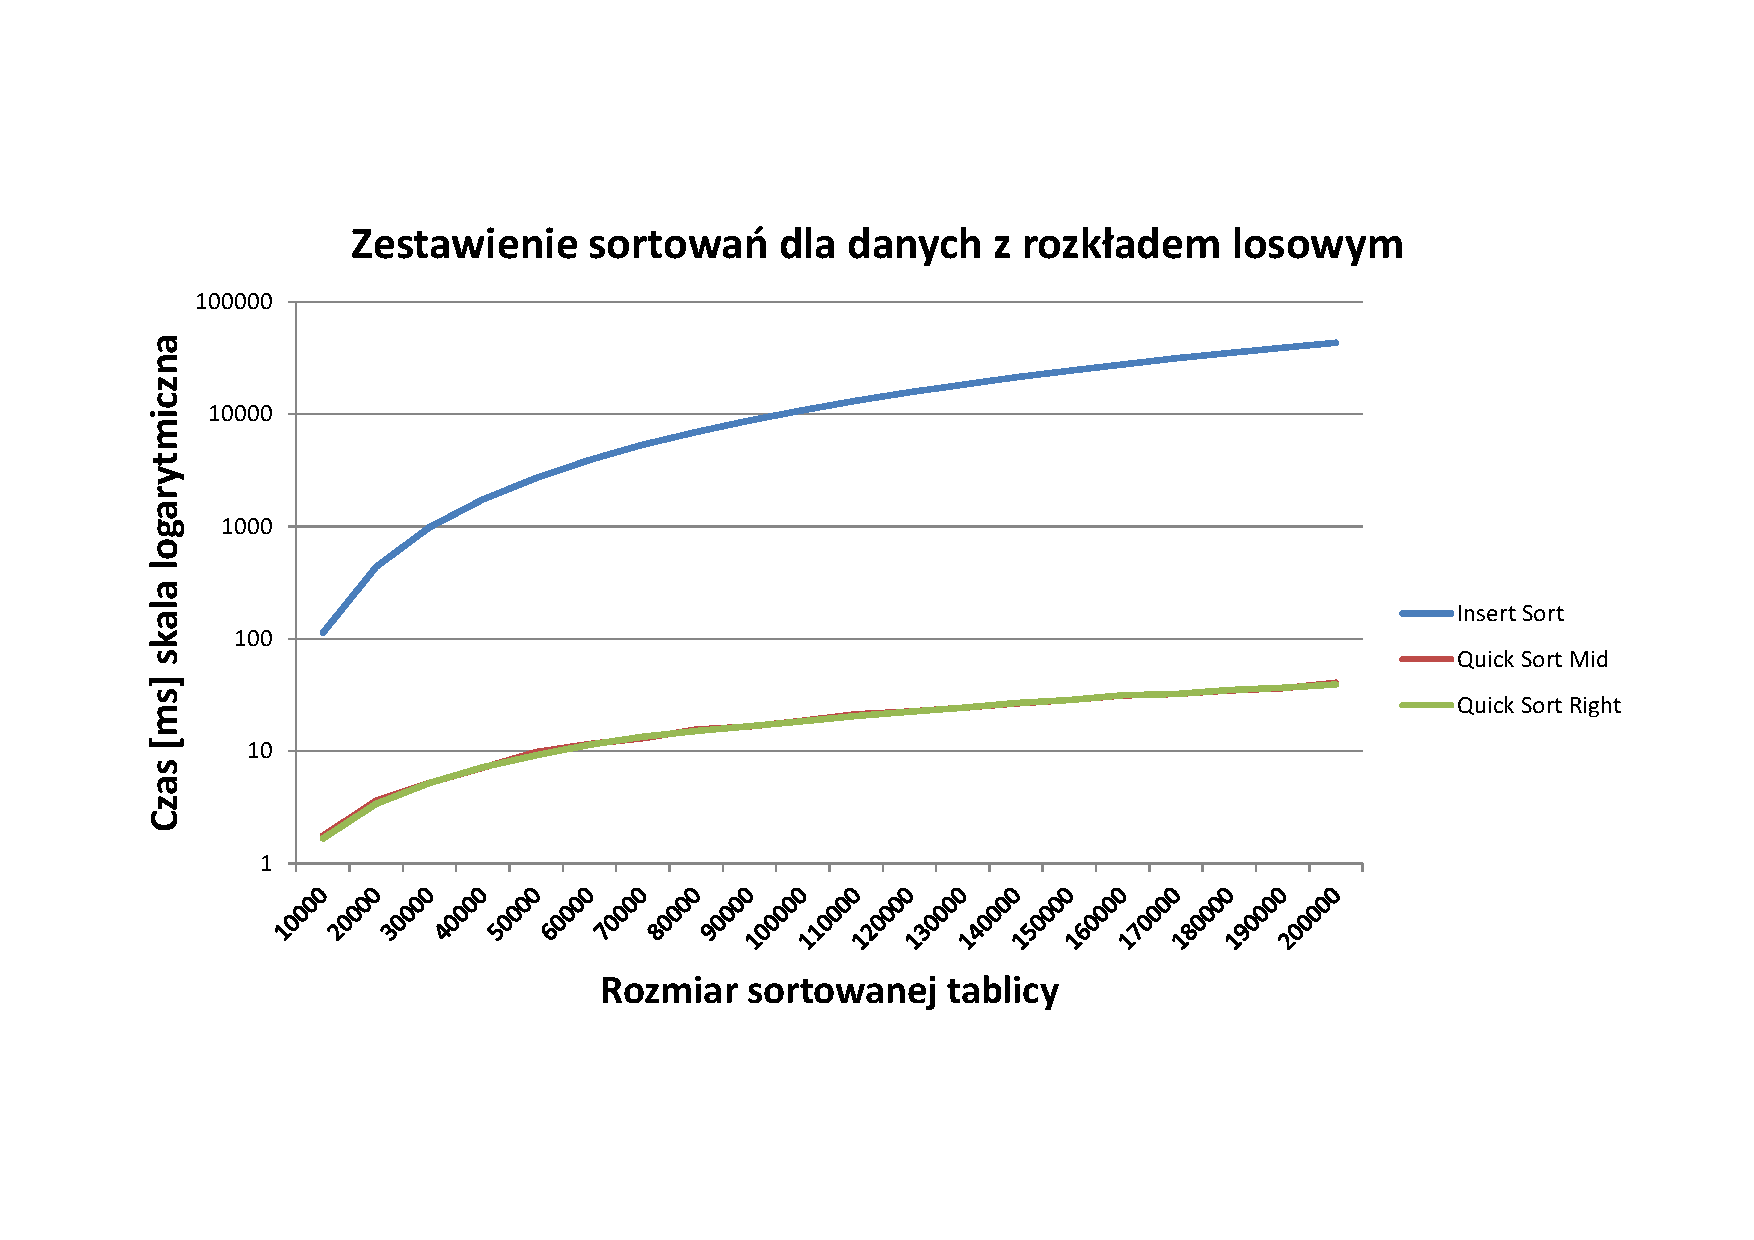
\includegraphics[scale=0.55]{zad3losowylog.pdf}
		\label{fig:zad3loslog}
	\end{center}
\end{minipage}


\subsection{Rozkład rosnący}

\subsubsection*{Wykresy ilustrujące zależności czasu sortowania od ilości elementów dla metod Quick Sort Mid, Quick Sort Right, Insertion Sort, dla rozkładu rosnącego.}


	

\begin{minipage}[H]{\textwidth}
	\begin{center}
		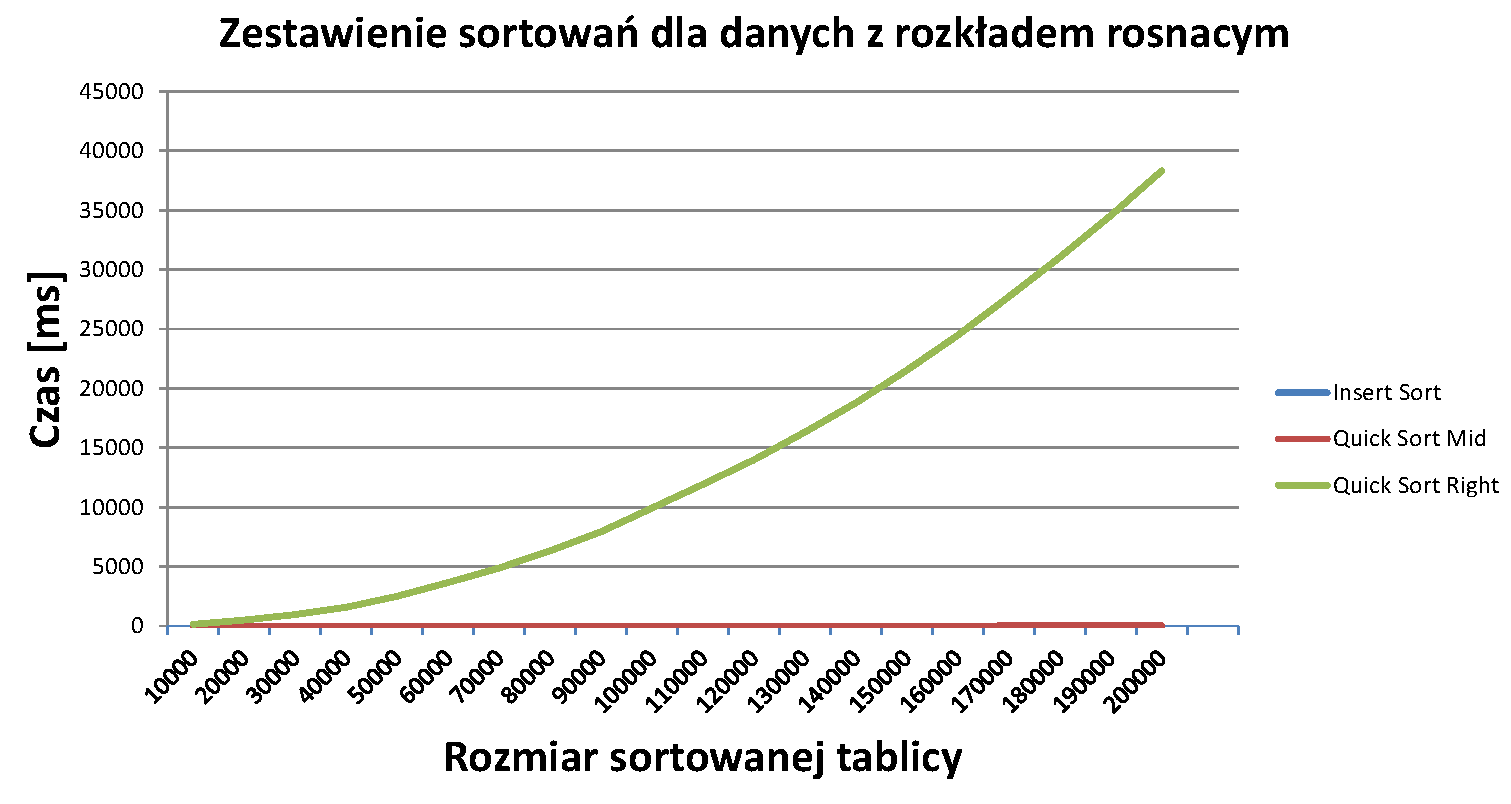
\includegraphics[scale=0.6]{zad3rosnacynorm.pdf}
		\label{fig:zad3rosn}
	\end{center}
\end{minipage}\\[1cm]



\begin{minipage}[H]{\textwidth}
	\begin{center}
		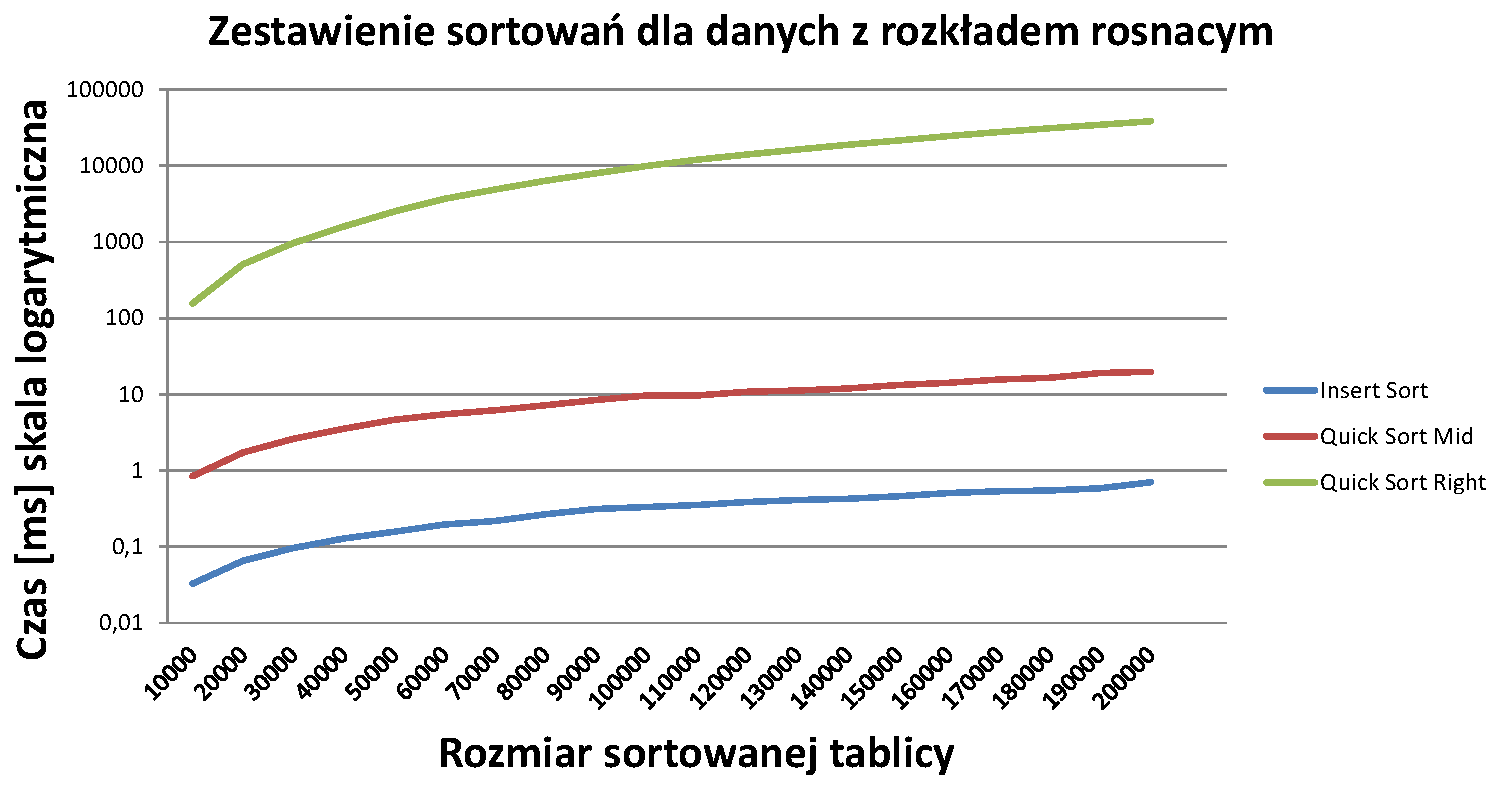
\includegraphics[scale=0.6]{zad3rosnacylog.pdf}
		\label{fig:zad3roslog}
	\end{center}
\end{minipage}


\subsection{Wnioski do zależności czasu $t$ od liczby sortowanych elementów $n$, przy rozkładach losowych i rosnących, dla metod Quick Sort z podziałem wg: skrajnego i środowego elementu, oraz dla metody Insert Sort}

Na złożoność obliczeniową Quick Sort-a wpływa punkt podziału tablicy. Można zauważyć, że ta metoda wykorzystująca skrajny element (w przeprowadzonym badaniu prawy) radzi sobie bez porównania gorzej niż ta, wybierająca środkowy dla tablicy, która ma rozkład danych rosnący. Najprawdopodobniej wynika to z tego, że wolniejszy algorytm (dla tego typu danych) zawsze dzieli rekurencyjnie zbiór danych na jednoelementowe podzbiory, przez co ilość nie posortowanych elementów zmniejsza się tylko o jeden. Co w konsekwencji prowadzi do wywołania większej ilości rekurencji. Ponadto warto zwrócić uwagę na fakt, że dla rozkładu losowego nie można wybrać jednoznacznie szybszej metody (w 12 na 20 przypadków szybszy był Quick Sort ze skrajnym podziałem tablicy, w pozostałych 8 ze środkowym elementem). Godnym uwagi wydaje się również spostrzeżenie, że Insert Sort pomimo niewspółmiernie gorszych wyników w stosunku do Quick Sort dla danych losowych, pozostawia go daleko w tyle dla danych o rozkładzie rosnącym. Z przeprowadzonego badania można wyciągnąć wnioski, że Quick Sort radzi sobie o niebo lepiej niż Insert Sort dla danych o rozkładzie losowym, jednakże sortowanie przez proste wstawianie nieporównywalnie szybciej przejdzie przez tablicę już uporządkowaną rosnąco.

Nie ma uniwersalnej metody sortowania dla każdego typu danych. Podczas wyboru algorytmu warto zwrócić uwagę na kilka aspektów. Pierwszym z nich jest zakres, z jakiego dane pochodzą, jeżeli jest on wąski, to najlepszym pomysłem będzie użyć Counting Sort-a, jednakże jeżeli pochodzi on z dużego zakresu, to ta metoda jest odradzana. Innym równie ważnym aspektem jest ilość zasobów, jakimi dysponujemy. Jeżeli nie mamy dodatkowej pamięci, przewagę zdobywają algorytmu sortujące w miejscu takie jak Insert Sort, Selection Sort czy Bubble Sort, z kolei, jeżeli ją posiadamy warto sięgnąć po metody bardziej wydajne np. Merge Sort. Kolejnym czynnikiem jest rozkład danych. Jeżeli posiadamy jakieś informacje o nim (np. czy jest rosnący, malejący lub losowy), możemy dobrać odpowiednią metodę, która przyspieszy czas trwania porządkowania informacji np. jeżeli wiemy, że dane są rosnące to rozsądnym wyborem będzie Quick Sort.

\section{Badanie zależności czasu obliczeń $t$ od liczby sortowanych elementów $n$ dla metod Counting Sort, Quick Sort, przy rozkaładzie losowym, gdy wartości elementów mieszczą się w przedziałach  $ [1;0,01n] $,$ [1;100n] $. }

\subsection{Przedział $[1;0,01n]$}

\subsubsection*{Wykres ilustrujący zależność czasu obliczeń od ilości elementów dla metod Counting Sort i  Quick Sort, dla rozkładu losowego w przedziale $[1;0,01n]$.}
	
	\begin{minipage}[H]{\textwidth}
		\begin{center}
			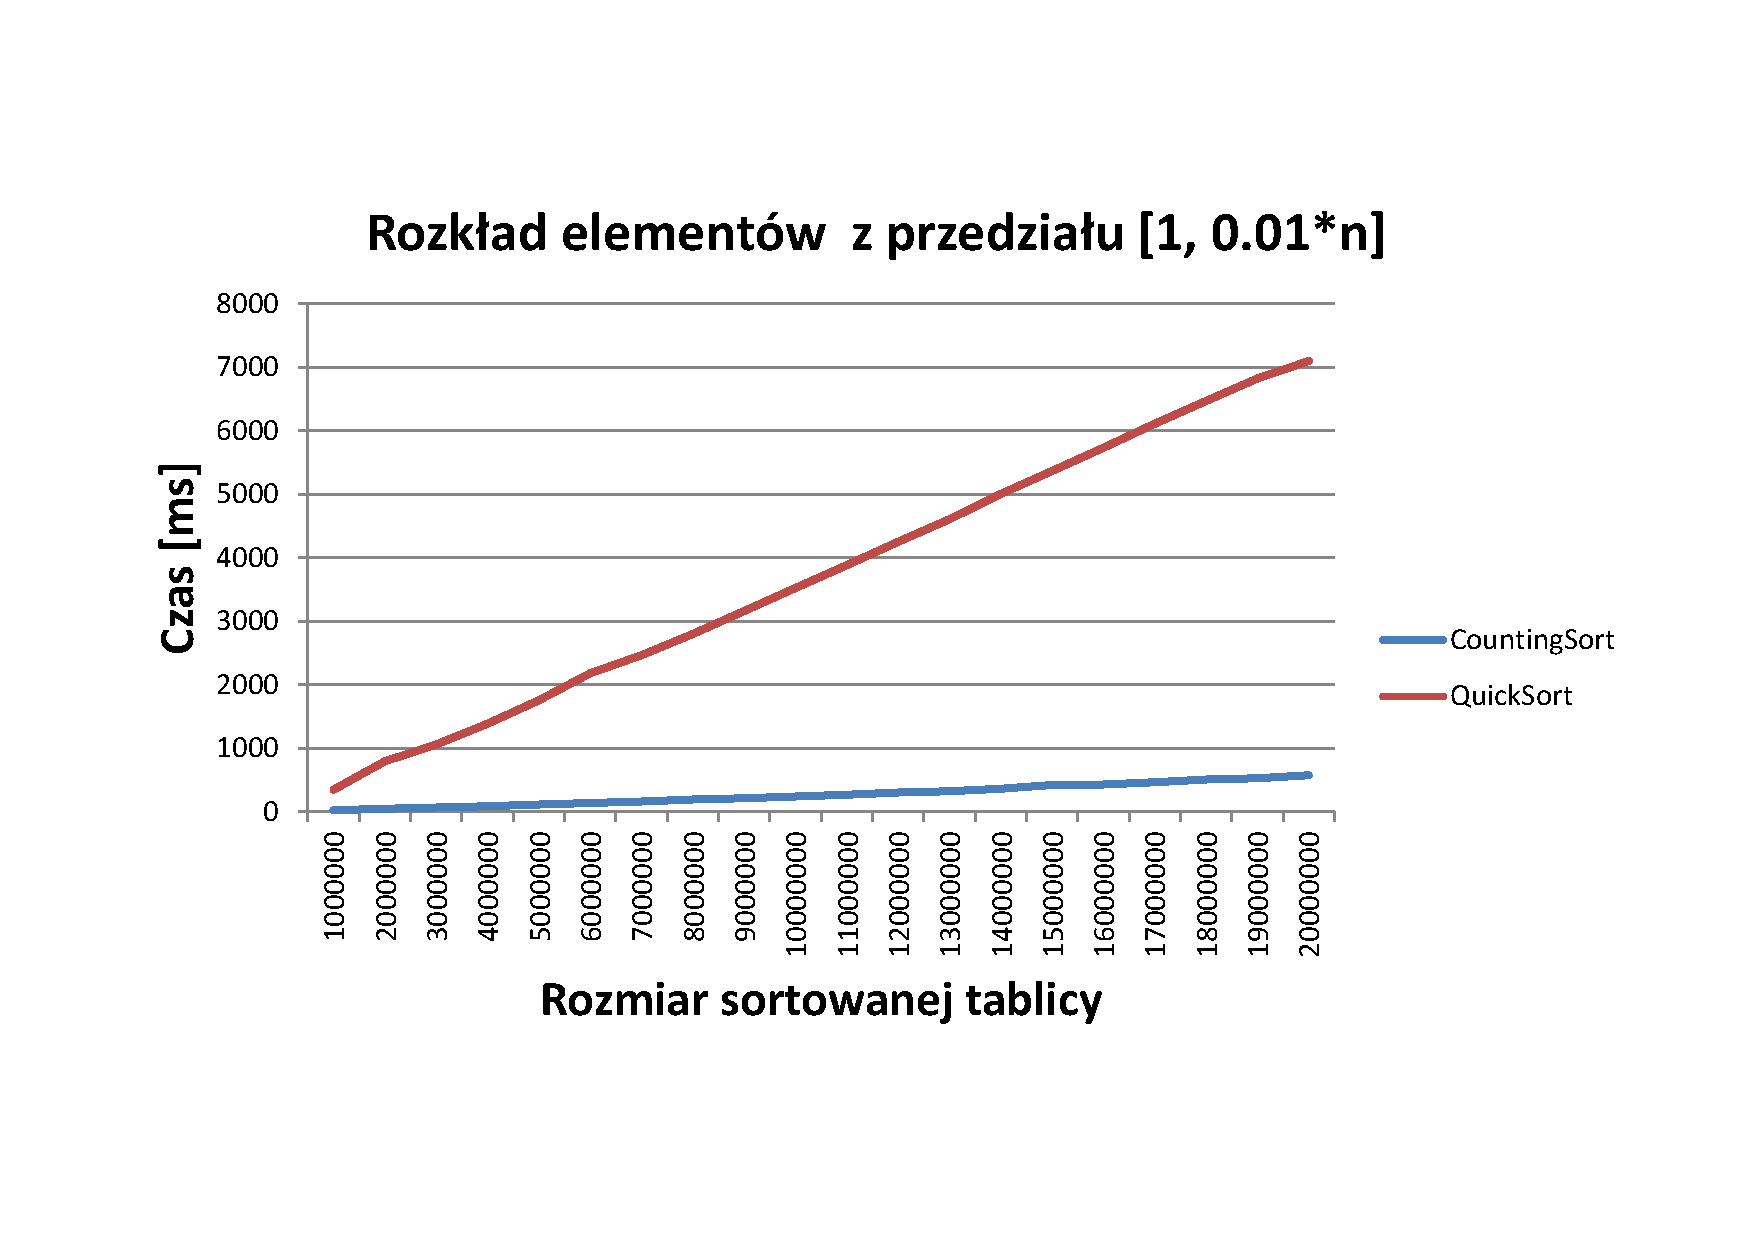
\includegraphics[scale=0.6]{zad4001n.pdf}
			\label{fig:zad4001n}
		\end{center}
	\end{minipage}

Badanie odbywało się w sposób następujący: wylosowanie tablicy do posortowania o rozmiarze $n$ z wartościami z przedziału $[1;0,01n]$, skopiowanie wylosowanej tablicy do tablicy pomocniczej, sortowanie metodą Quick Sort z pomiarem czasu, przywrócenie posortowanej tablicy do stanu przed sortowaniem przy użyciu tablicy pomocniczej, sortowanie metodą Counting Sort z pomiarem czasu, zwiększenie rozmiaru $n$ i ponowne przeprowadzenie całego procesu, do momentu aż $n$ osiągnie pożądaną wartość.	Dzięki takiemu rozwiązaniu w sekcji Diagnostic Tools programu Visual Studio 2015 można było obserwować zauważalny  wzrost zużywanej pamięci podczas metodą sortowania przez zliczanie, w porównaniu do ilości pamięci używanej w trakcie sortowania metodą szybką.

\subsubsection*{Zrzut ekranu sekcji Diagnostic Tools programu Visual Studio 2015 prezentujący, zużycie pamięci i procesora w trakcie sortowania algorytmami Counting Sort i  Quick Sort, dla rozkładu losowego w przedziale $[1;0,01n]$.}

	\begin{minipage}[H]{\textwidth}
	\begin{center}
		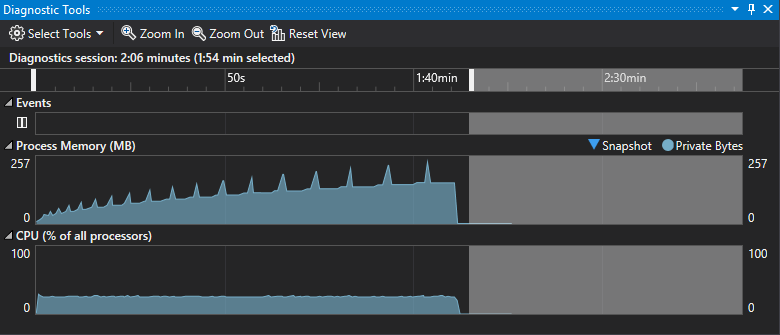
\includegraphics[scale=0.85]{zad4pamiec001n.png}
		\label{fig:zad4pamiec001n}
	\end{center}
	\end{minipage}

\subsubsection{Wnioski do przedziału $[1;0.01n]$}

Po przeanalizowaniu wyników badania można zauważyć że metoda sortowania przez zliczanie działa znacznie szybciej niż Quick Sort w przedziale $[1;0,01n]$, przy trochę większym wykorzystaniu pamięci. Metoda Counting Sort sprawdza się lepiej przy sortowaniu tablic z małym zakresem liczb od metody szybkiej, co czyni ją efektywniejszą, ale tylko w przypadku kiedy mamy wystarczającą ilość pamięci przeznaczonej dla procesu.

\subsection{Przedział $[1;100n]$}

\subsubsection*{Wykres ilustrujący zależność czasu obliczeń od ilości elementów dla metod Counting Sort i  Quick Sort, dla rozkładu losowego w przedziale $[1;100n]$.}

\begin{minipage}[H]{\textwidth}
	\begin{center}
		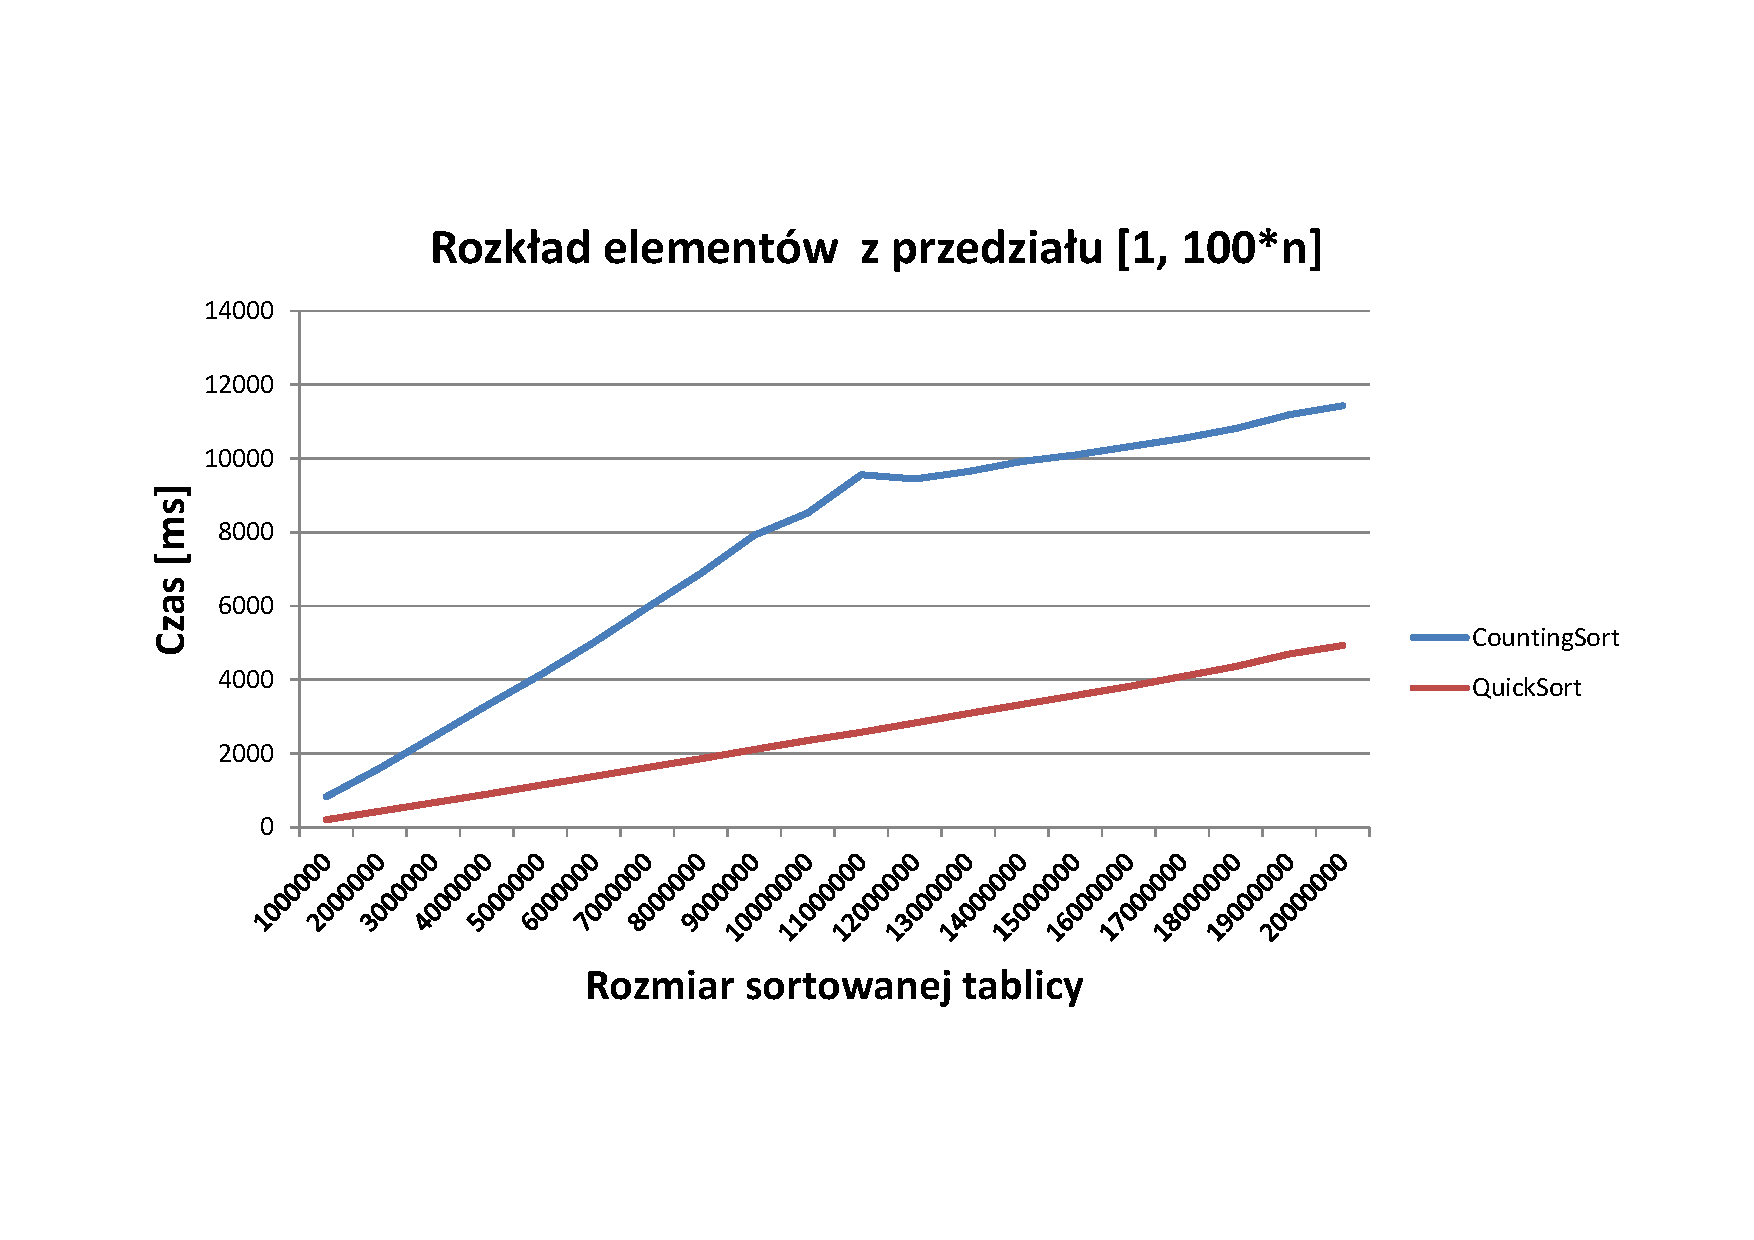
\includegraphics[scale=0.6]{zad4100n.pdf}
		\label{fig:zad4100n}
	\end{center}
\end{minipage}\\

Badanie odbywało się w sposób następujący: wylosowanie tablicy do posortowania o rozmiarze $n$ z wartościami z przedziału $[1;100n]$, skopiowanie wylosowanej tablicy do tablicy pomocniczej, sortowanie metodą Quick Sort z pomiarem czasu, przywrócenie posortowanej tablicy do stanu przed sortowaniem przy użyciu tablicy pomocniczej, sortowanie metodą Counting Sort z pomiarem czasu, zwiększenie rozmiaru $n$ i ponowne przeprowadzenie całego procesu, do momentu aż $n$ osiągnie pożądaną wartość.	Dzięki takiemu rozwiązaniu w sekcji Diagnostic Tools programu Visual Studio 2015 można było obserwować nagły wzrost zużywanej pamięci podczas metodą przez zliczanie, w porównaniu do ilości pamięci używanej w trakcie sortowania metodą szybką. 

\subsubsection*{Zrzut ekranu sekcji Diagnostic Tools programu Visual Studio 2015 prezentujący, zużycie pamięci i procesora w trakcie sortowania algorytmami Counting Sort i  Quick Sort, dla rozkładu losowego w przedziale $[1;100n]$.}

\begin{minipage}[H]{\textwidth}
	\begin{center}
		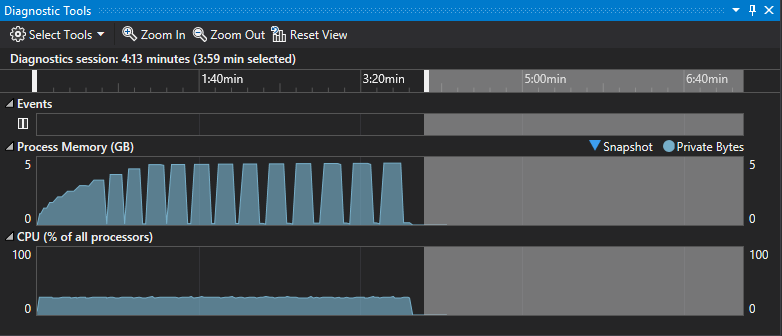
\includegraphics[scale=0.85]{zad4pamiec100n.png}
		\label{fig:zad4pamiec100n}
	\end{center}
\end{minipage}



\subsubsection{Wnioski do przedziału $[1;100n]$}

Po przeanalizowaniu wyników badania można zauważyć że metoda Quick Sort działa znacznie szybciej niż Counting Sort w przedziale $[1;100n]$, przy pioruńsko większym (w niektórych przypadkach nawet dwudziestokrotnie) wykorzystaniu pamięci. Metoda szybka sprawdza się lepiej przy sortowaniu tablic z dużym zakresem liczb od metody przez licznie, co czyni ją efektywniejszą.


\subsection{Wnioski do badania zależności czasu obliczeń $t$ od liczby sortowanych elementów $n$ dla metod Counting Sort, Quick Sort, przy rozkładzie losowym, gdy wartości elementów mieszczą się w przedziałach  $ [1;0,01n] $,$ [1;100n] $. }

Po przeprowadzeniu badana jasno widać jak ważne jest dobranie odpowiedniej metody sortowania dla swoich danych. Na efektywność użytej metody ma wpływ między innymi przedział elementów. W przypadku kiedy pracujemy na mniejszym przedziale warto wybrać metodę sortowania przez zliczanie, jeżeli posiadamy wystarczającą ilość pamięci. Przy większym przedziale metoda Quick Sort staje się efektywniejsza, Counting Sort nie tylko działa wolniej, ale też zużywa wielokrotnie więcej pamięci.
	

	
\end{spacing}
	\newpage
	\tableofcontents
\end{document}


